\chapter{Big Data, NoSQL, Testes de Software e Web Services}

Este capítulo traz uma contextualização sobre quatro temas relevantes ao trabalho. \emph{Big Data} e \emph{NoSQL} são os alicerces tecnológicos que motivaram nossa investigação, que considera alternativas recentes de armazenamento, tipicamente encontradas em bancos de dados não relacionais, e que suportam grandes volumes de dados (características de ambientes de \emph{Big Data}). Como o alvo da pesquisa está relacionado ao desempenho no processamento das requisições, contextualizamos a área de testes de software que tem como um dos alvos a análise de desempenho de sistemas. O protótipo arquitetural foi baseado em uma arquitetura orientada a serviços ~\cite{erl:2007} que disponibiliza algumas das principais capacidades para manter os dados do AFD, sendo assim, será discutido também os principais conceitos de \textit{Web services}.

\section{Big Data}


A quantidade de informação que está disponível para a humanidade é enorme e a medida que o conhecimento humano se expande, maior é a quantidade dessa informação que precisa ser armazenada e analizada. Além da quantidade, o fluxo e variedade dessas informações constantemente desafiam a indústria e a academia a medida em que a quantidade de \textit{big  data} aumenta exponencialmente. Essa seção apresenta uma definição detalhada de o que é \textit{big data} e as tecnologias que apoiam esse domínio.

\subsection{O que é Big Data?}

Em um estudo divulgado em 2011 o tamanho do universo digital quebrou a barreira dos \textit{zettabytes} e esse número está crescendo rapidamente~\cite{emcuniversedigital}. Cientistas de diversas áreas estão vendo o grande potencial de conhecimento que se pode adiquirir pela análise a armazenamento de informação digital. Conforme já dito anteriormente o conceito de ``grande (\textit{big})''  evoluiu no decorrer da nossa história. Na década de 70, grande significava \emph{kilobytes}; ao longo do tempo cresceu para \emph{gigabytes} e em seguida, a \emph{terabytes}. Atualmente já podemos dizer que grande varia de \emph{petabytes}  até \emph{exabytes}~\cite{WNextBigData}. Contudo  o  conceito de \textit{big data} não se dá somente por tamanho ou domínio, mas também por um conjunto de características que o difere de uma base de dados comum.

Segundo o Gartner \emph{big data} é definido, em geral, como uma massa de dados de grande volume, velocidade e variedade de informações que exigem formas inovadoras de processamento para maior visibilidade e tomada de decisão~\cite{conceitoGartner}. A maioria dos estudiosos compartilham dessa mesma definição e afirmam que \textit{big data} é caracterizado por no mínimo três V's. Volume, variedade e  velocidade.~\cite{ibmbigdatavvv,fromdbtobigdata}

Volume é a característica mais fácil de se perceber. Geramos enormes quantidades de dados todos os dias, e essa quantidade só tende a aumentar. Redes sociais, dispositivos móveis que guardam nossas informações, sites que armazenam nossas preferências, dispositivos de busca que indexam as páginas da web e a popularização da computação em nuvem nos colocam em uma época de grande volume de dados, uma época em que tudo é informação, tudo é valioso, tudo pode ser extraído. Cada dia fica mais comum grandes empresas terem de lidar com dados na ordem de \textit{petabytes}. Variedade é outra característica que é de fácil percepção, pois os dados são de diversas naturezas como email, dados gerados por mídias sociais (\textit{blogs}, Twitter, Youtube, Facebook, \textit{Wikis}), documentos eletrônicos, apresentações, fotos, mensagens instantâneas, dados médicos, videos, etc. A característica de velocidade é explicada quando precisamos processar os dados praticamente em tempo real como em controle de tráfego, detecções de fraudes e propagandas dinâmicas na web. Os dados são cada vez mais usados para tomadas de decisão em tempo real~\cite{promiseperil}.

\begin{table}
	\caption{Tabela de bytes}
	\begin{center}
	\begin{tabular}{ccc}
		\hline
			\textbf{Nome} & \textbf{Tamanho} & \textbf{Abreviação} \\
		\hline
			\texttt{Kilobyte}	& $10^3$ & KB \\
			\texttt{Megabyte}	& $10^6$ & MB \\
			\texttt{Gigabyte}	& $10^9$ & GB \\
			\texttt{Terabyte}	& $10^{12}$ & TB \\
			\texttt{Petabyte}	& $10^{15}$ & PB \\
			\texttt{Exabyte}	& $10^{18}$ & EB \\
			\texttt{Zettabyte}	& $10^{21}$ & ZB \\
			\texttt{Yottabyte}	& $10^{24}$ & YB \\
		\hline
	\end {tabular}
	\end{center}
	\label{tab:bytes}
\end{table}

Dada a problemática do armazenamento, ao se deparar com os limites de técnicas e ferramentas disponíveis, o mercado tratou de criar suas próprias soluções de gerenciamento de dados, em sua maioria não relacional. Usando a tecnologia apropriada, profissionais capacitados podem transformar grandes massas de dados em informações muito valiosas. Muitos sistemas comercias relacionais se dizem capazes de lidar com vários \textit{petabytes} de base de dados (Greenplum, Netezza, Teradata, ou Vertica). Apesar dessa quantidade de dados atender a grande maioria das empresas, existem empresas de grande porte como o Google e o Facebook que não são atendidas e precisaram criar suas próprias soluções, além disso, sistemas \textit{open source} como Postgres  não tem o mesmo nível de escalabilidade que os comerciais ~\cite{fromdbtobigdata}.
%Dado isso, foram surgindo alternativas ao Modelo Relacional das quais a que mais se destacou foi o paradigma NoSql.(tcc-gleison)

\subsection{Bases de dados relacionais}

Quando pensamos em armazenamento de dados em SGBDs logo associamos essa ideia ao método tradicional que inclui bancos de dados como MySQL, PostgreSQL, modelagem relacional e esquemas de dados bem definidos. O modelo de dados relacional foi introduzido por Ted Codd, da IBM Research, em 1970, em um artigo que conseguiu atrair grande atenção devido à simplicidade e base matemática. Os SGBDs relacionais mais populares atualmente são o DB2 e Informix Dynamic Server (IBM), o Oracle e Rdb (Oracle), o Sybase SGBD (Sybase) e o SQLServer e Access (Microsoft). Ainda temos os de código aberto como o MySQL e PostgreSQL.

O modelo relacional representa o banco de dados como uma coleção de relações \ref{fig:modelorelacional}. Uma relação é similar a uma tabela de valores ou um arquivo de registros. Cada tabela é formada por uma ou mais colunas de dados. Por sua vez, cada linha na tabela contém uma instância única de dado para as categorias de colunas definidas. No modelo relacional é possível criar conexões entre as tabelas e os  campos e os formatos dos valores são bem definidos, ou seja, possui um \textit{schema} de dados~\cite{SBElmasri,nosqlliveup}.

	\begin{figure}[!htbp]
		\begin{center}
			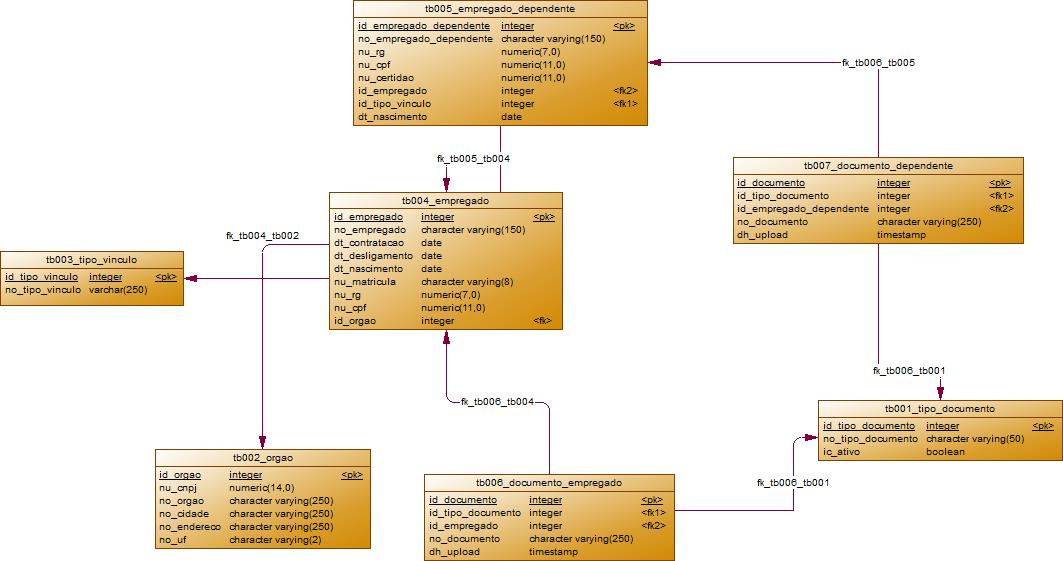
\includegraphics[width=0.8\textwidth]{modelo_relacional}
		\end{center}
		\caption{Modelo Relacional }
		\label{fig:modelorelacional}
	\end{figure}

Umas das características mais importantes das bases de dados relacionais são as garantias das propriedades ACID  ~\cite{Orendanalysisand}. ACID é um acrônimo para \textit{Atomicity}(Atomicidade), \textit{Consistency}(Consitência), \textit{Isolation} (Isolamento) e \textit{Durability} (Durabilidade).
Atomicidade significa que todas as etapas de uma transação serão executadas, caso contrário a transação será abortada sem interferir no banco de dados. Consistência significa que um banco de dados estará em um estado consistente antes e após cada transação. Caso as mudanças de uma transação violarem a regra de consistência, então todas as mudanças serão revogadas para garantir que somente os dados realmente válidos serão escritos no banco de dados. Isolamento, por sua vez, significa que as transações não podem visualizar as mudanças que não foram submetidas ao banco. Como as alterações que resultaram em erros. Finalmente, a propriedade de durabilidade requer que os dados sejam escritos no banco antes da transação ser confirmada. Caso haja uma falha de energia os dados não serão perdidos.

Os SGBDs (Sistemas Gerenciadores de Banco de Dados) relacionais proveem diversas garantias aos seus usuários, como validação, verificação e garantias de integridade dos dados, controle de concorrência, recuperação de falhas,  entre outros. Todas essas características mantém os SGBDs como principal solução na maioria dos ambientes computacionais, mas não impediram o surgimento de problemas, em alguns casos, causados pela rígida estrutura definida pelo \textit{layout} das tabelas, nomes e tipos das colunas.

As abordagens mais usadas para manipular grandes bases nesse tipo de estrutura são os \textit{data warehouses} e \textit{data marts}. Um \textit{data warehouse} é um banco de dados relacional usado para armazenar, analizar e gerar relatórios sobre os dados. O \textit{data mart} é a camada usada para acessar o \textit{data warehouse}. As duas abordagens usadas para se armazenar dados em um \textit{data warehouse} são a normalização e a modelagem dimensional~\cite{bigdataarchitectureandapproach}.

Por outro lado, com a evolução das aplicações e com requisitos cada vez mais exigentes, foram surgindo casos em que os bancos de dados relacionais não escalavam. Operações de \textit{joins} estão presentes nos menores dos bancos de dados relacionais, e esse tipo de operação é lenta. Para que SGBDs relacionais consigam garantir consistência para os dados eles usam o conceito de transações, o que requer um bloqueio nos dados durante um certo período de tempo.  Dessa forma, quando o banco recebe várias requisições simultâneas em um mesmo dado os usuários são obrigados a esperarem em uma fila~\cite{cassandraguide}.

A necessidade de transformar os dados em tabelas causa um aumento na complexidade da operação, pois requer o uso de complexos algoritmos de mapeamento e estrutura. Mesmo quando uma base de dados pode ser coberta pelo modelo relacional, às vezes as diversas garantias providas por esse modelo gera uma sobrecarga que não seria necessária para tarefas simples. O \textit{schema} rigoroso pode ser pesado para aplicações que precisam de velocidade, como aplicações web e \textit{blogs} que possuem diversos tipos de atributos. Textos, comentários, imagens, vídeos, código fonte e outras informações precisam ser armazenadas em diversas tabelas, e como as aplicações na web são muito ágeis, precisam ser amparadas por uma base de dados igualmente ágil e com um ztextit{schema} de fácil adaptação ~\cite{nosqlevaluation}.

O considerável aumento na quantidade de dados deve ser considerado por grandes empresas como Facebook, Amazon e Google. Além de tratar \textit{terabytes}/\textit{petabytes} de dados, realizar requisições de leitura e escrita na base a todo o momento essas empresas devem se preocupar com o tempo que essas transações estão levando, ou seja, a latência. Para tratar esses requisitos é preciso manter milhares de máquinas com um \textit{hardware} moderno e veloz. Por ter que cumprir com os requisitos de ACID e manter os dados normalizados, um modelo relacional não é adequado para esse cenário, visto que as operações de \textit{join} bloqueiam os dados e influenciam negativamente no desempenho da aplicação.

Outro requisito fundamental para as grandes empresas é a disponibilidade de seus serviços. Para isso a base de dados deve ser facilmente replicável e fornecer uma forma automática de tratamento à falha de bases ou do \textit{datacenter}. Esses SGBDs também devem ser capazes de balancear a carga em várias máquinas para não sobrecarregar um único servidor. Bancos relacionais priorizam a consistência em detrimento à disponibilidade e também possuem um mecanismo de replicação limitado.

Esses problemas podem ser resolvidos de algumas formas.Primeiramente optamos por um \textit{upgrade} simples de \textit{hardware}. Se o problema persistir a próxima opção seria adicionarmos novos servidores ao \textit{cluster}, porém com os problemas de consistência e replicação durante o uso regular e em cenários de falha. A próxima etapa seria melhorar a configuração do gerenciador de banco de dados. Caso as opções de melhoria no SGBD se esgotem é preciso melhorar a aplicação. Verifica-se o desempenho das consultas, criamos índices e etc. Se o desempenho ainda não for satisfatório então talvez coloquemos uma camada de \textit{cache}, mas que também gera um problema de consistência. Se mesmo assim o desempenho não atender as expectativas, então é necessário pensarmos novamente no SGBD. A última opção seria uma desnormarlização do banco, mas assim se estaria indo contra os princípios da modelagem relacional e das regras normais~\cite{cassandraguide}.

Dado toda essa problemática surge uma opção. Bancos de dados que não seguem o paradigma relacional. Os dados não são normalizados.

\subsection{Bases Não Relacionais}

O NoSQL foi proposto em 2009 e quebrou os limites das bases de dados relacionais e das propriedades ACID. Os bancos de dados NoSQL geralmente não proveem as propriedades ACID: atualizações são eventualmente propagadas, mas há garantias limitadas para a consistência de leituras. Alguns autores sugeriram  o acrônimo ‘BASE’ em contraste ao ‘ACID’ ~\cite{scalablesqlandnosql}. O teorema CAP, o teorema BASE e o conceito de consistência eventual são os fundamentos do NoSQL, discutidos no decorrer dessa seção.

\subsubsection{Teorema CAP}

O teorema CAP (Figura \ref{fig:captheorem}) foi proposto por Eric Brewer. CAP significa Consistência,  disponibilidade e tolerância a particionamento de rede.  A idéia principal desse teorema é que os sistemas distribuídos não podem atender, ao mesmo tempo, essas três características. Podem atender somente duas delas ~\cite{nosqlaplicassandra}.

	\begin{figure}[!htbp]
		\begin{center}
			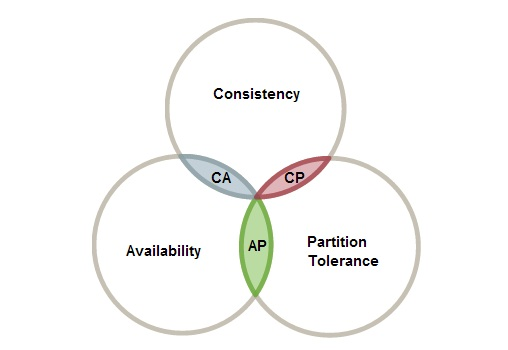
\includegraphics[width=0.8\textwidth]{captheorem}
		\end{center}
		\caption{Teorema CAP ~\cite{capimage} }
		\label{fig:captheorem}
	\end{figure}

Nesse caso a disponibilidade permite que os clientes sempre possam executar leituras e escritas em um certo período de tempo. Um banco de dados distribuído que permite particionamento é tolerante à falhas de conexão e permite a distribuição em nós separados ~\cite{Orendanalysisand}.

Um sistema que permite o particionamento só poderá prover uma consistência forte se sacrificar a disponibilidade. Isso porque cada operação de escrita somente será concluída se os dados forem replicados para todos os nós, o que nem sempre é possível em um ambiente com falhas de conexão ou outras falhas de \textit{hardware} ~\cite{Orendanalysisand}.

Sendo assim, temos três arquiteturas possíveis: CA, AP e CP. Como atualmente a grande maioria dos sistemas é implantada na web, a disponibilidade é indispensável. Isso nos permite utilizar somente com as arquiteturas CA e AP. Para sistemas web, a disponibilidade e a tolerância ao particionamento são mais importantes que a consistência. Já é suficiente quando um sistema web possui consistência eventual ~\cite{nosqlaplicassandra}.

\subsubsection{Teorema BASE}

O teorema BASE é um produto do teorema CAP. As propriedades BASE são completamente diferentes das ACID. BASE é um acrônimo para: \textit{Basically Available} (Basicamente Disponível), \textit{Soft-state}(base otimizada pelo uso) e \textit{Eventual consistency} (Disponibilidade Eventual) ~\cite{nosqlaplicassandra}.

\begin{itemize}
\item \textit{BasicallyAvailable} : Significa que eventuais falhas de particionamento são suportadas.
\item \textit{Soft-state}: Significa que em um período de tempo o estado do sistema pode ser assíncrono.
\item \textit{Eventual consistency}: O sistema ‘deve’ ser consistente.
\end{itemize}

\subsubsection{Consistência Eventual}

Por causa o teorema CAP, a maioria dos banco de dados NoSQL proveem consistência eventual. Abaixo estão as definições de consistência forte e consistência eventual.

Consistência forte: Significa que todos os processos conectados em um banco de dados sempre verão a mesma versão de um valor e uma nova atualização é instantaneamente refletida por qualquer operação de leitura até outra mudança ser feita por outra operação de escrita ~\cite{Orendanalysisand}. Na Figura \ref{fig:strongconsistency} temos um exemplo gráfico.

	\begin{figure}[!htbp]
		\begin{center}
			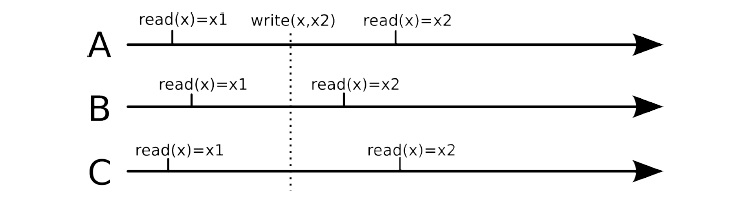
\includegraphics[width=0.8\textwidth]{strongconsistency}
		\end{center}
		\caption{Consistência Forte: O processo A, B e C sempre estão vendo a mesma versão do banco de dados ~\cite{Orendanalysisand}.}
		\label{fig:strongconsistency}
	\end{figure}

Consistência Eventual: É um tipo de consistência fraca. O não garante que todos os processos veem a mesma versão dos dados. Isso pode ocorrer por causa das janelas de inconsistência e é geralmente causada pela replicação dos dados nos diferentes nós ~\cite{Orendanalysisand}. Na Figura \ref{fig:eventualconsistency} temos um exemplo gráfico.

	\begin{figure}[!htbp]
		\begin{center}
			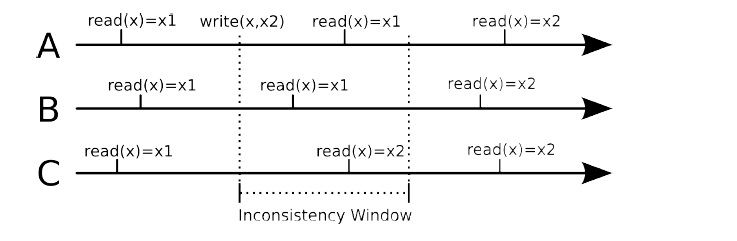
\includegraphics[width=0.8\textwidth]{eventualconsistency}
		\end{center}
		\caption{Consistência Eventual: Os processos A, B e C podem visualizar diferentes versões dos dados durante a janela de inconsistência causada pela replicação assíncrona ~\cite{Orendanalysisand}.}
		\label{fig:eventualconsistency}
	\end{figure}








\chapter{NoSql}

Nesse capítulo iniciaremos com a definição de o que é o termo NoSQL e, após vermos como essa nova forma de se pensar em banco de dados surgiu, conheceremos os principais tipos de banco de dados não relacionais e como eles armazenam os seus dados. 


\section{Definição de NoSQL}

O termo NoSql é a junção de duas palavras. No and SQL. Ao pé da letra significa que é uma tecnologia/produto que trabalha de forma contrária à tecnologia dos banco relacionais (adeptos do SQL). O termo é usado com o sentido de Não Relacional. Atualmente o termo NoSql é traduzido para "Not only Sql", ou seja "Não só Sql".
Saindo da definição, NoSql é um termo genérico para uma classe definida de banco de dados não-relacionais que armazenam os dados  de forma diferente da conhecida modelagem relacional e que surgiram com o propósito de sanar algumas dificuldades encontradas com o modelo relacional. NoSql não é um produto, mas a uma classe de produtos e conceitos de armazenagem e manipulação de dados. 

O que diferencia os bancos de dados NoSql dos relacionais são os seus modelos de dados sem um schema definido. Os bancos de dados NoSql podem ser classificados, segundo seu modelo de dados, em quatro grupos: chave-valor, orientados a documentos, orientados a colunas e baseados em grafos~\cite{nosqlxrelacional,nosqlevaluation}.

\section{História}

Bancos de dados que usam a modelagem não relacionais não são novidades. Conforme discutido no livro (NoSql Professional) eles surgiram junto com as primeiras máquinas de computar. Bases não relacionais ficaram conhecidas e cresceram por causa do uso de mainframes e em dominios específicos como o armazenamento de credenciais para autenticação. Esse NoSql que conhecemos hoje é uma nova visão, ou como diz fulano em (NoSql Professional), uma reincarnação que nasceu no mundo de aplicações web que necessitam de recursos escaláveis para tratar de sua enorme massa de dados. Apesar de o paradigma NoSql já ter sido criado há algum tempo nenhum ele só tomou as proporções atuais depois que grandes empresas como Google, Amazon e Facebook começam a usar em suas arquiteturas~\cite{nosqlevaluation}.

Ao utilizar SGBD's relacionais com grandes quantidade de dados surgem problemas como falta de eficiência no processamento, uma paralelização não efetiva, alto custo e scalabilitade limitada. Sendo um gigante da internet, o Google,  se não for a empresa que manipula a maior quantidade de dados, é com certeza uma das maiores e ao se deparar com essa problemática  construiu a sua própria infraestrutura para que o seu mecanismo de busca e outras aplicações pudessem tratar a massa de dados de forma eficiente.

Com o lançamento de artigos pelo Google que explicavam em partes como o problema foi solucionado, desenvolvedores de software livre criaram o primeiro motor de busca de código aberto que replicava algumas característica da infraestrutura do Google, o Lucene. Logo depois, os principais desenvolvedores do Lucene se juntaram ao Yahoo e com a ajuda de diversos outros desenvolvedores criaram uma estrutura que imitada todas as peças da infraestrutura de computação distribuida do 
Google. Essa solução livre é o Hadoop. Nessa mesma época surgiu a idéia do NoSql. 

O sucesso do Google e o Hadoop ajudaram a impulsionar novos conceitos de computação distribuída, NoSql e o próprio projeto Hadoop. Um ano após o lançamento dos artigos do Google outra gigante da internet resolveu compartilhar o seu caso de sucesso. Em 2007 a Amazon mostrou ao mundo sua solução de base de dados distribuída, disponível e consistente que se chama Dynamo.

Após Google e Amazon mostrarem para o mundo que o NoSql dava certo começaram a surgim diversos outros produtos nessa linha. O NoSql e os conceitos de manipulação de Big Data ganharam espaço e forma surgindo diversos casos de uso de sucesso de grandes companias como o Facebook, Netflix, Yahoo, EBay, Hulu, IBM e diversas outras.



\section{Os Principais Tipos de Banco de Dados NoSql}


\subsection{Chave-Valor}

Bancos de dados NoSql que usam a modelagem Chave-Valor armazenam os dados indexados por um valor chave. A base é similar a um dicionário, onde os dados são endereçados por uma única chave. Uma vez que os dados são armazenados, é através das suas chaves a única forma de recuperá-los. Os valores sao isolados e independentes um dos outros, sendo necessário tratar isso na aplicação. Por isso banco chave-valor são livres de schema. Isso permite que novos tipos de dados sejam inseridos em tempo de execução sem que o banco entre em conflito e sem influenciar na disponibilidade do sistema~\cite{nosqlevaluation,nosqlliveup}.

Alguns exemplos de banco de dados que usam esse tipo de modelagem são: RIAK, LevelDB, Voldemort, redis~\cite{nosqldatabaseorg}.

\subsection{Orientados a Documentos}

A modelagem orientada a documentos armazena os dados encapsulados em pares de chave-valor em JSON ou em outro padão semelhante. Dentro dos documentos as chaves devem ser únicas. Cada documento recebe um identificador que também é único dentro de uma coleção de documentos. Os documentos são as unidades básicas e não têm uma estrutuda definida como nas tabelas do modelo relacional, ou seja, não tem um schema de dados definido. Ao armazenar os dados em JSON há uma vantagem adicional que é o suporte a tipos de dados, o que torna a forma de armazenamento mais amigavel para os desenvolvedores~\cite{nosqlevaluation,nosqlxrelacional}.

Os exemplos mais significativos são: CouchDB, MongoDB e Riak~\cite{nosqlevaluation}.

	\begin{lstlisting}[caption=Exemplo de arquivo do CouchDB]
{
    "Subject": "I like Plankton",
    "Author": "Rusty",
    "PostedDate": "5/23/2006",
    "Tags": ["plankton", "baseball", "decisions"],
    "Body": "I decided today that I don't like baseball. I like plankton."
}
	\end{lstlisting}

\subsection{Orientados a Colunas}

Nesse tipo de modelagem o paradigma passa a ser de orientação a atributos(colunas).Ao contrário da modelagem chave-valor, agora os dados são armazenados usando tabelas sem um schema definido, mas sem suporte a associação entre elas . Figura ~\ref{fig:mdcolumns} Segundo Jing Han et all, um banco orientado a colunas tem as seguintes caracteristicas ~\cite{surveynosql}:


\begin{enumerate}
\item{Os dados são armazenados em colunas}
\item{Cada coluna de dado é um índice do banco}
\item{Acessar somente colunas faz com que haja redução de I/O nos resultados das consultas}
\item{Consultas simultâneas, isto é, cada coluna é tratada por um processo}
\item{Possuem o mesmo tipo de dados, características semelhantes e boa taxa de compressão}
\end{enumerate}

Em geral esse tipo de banco é mais vantajoso para aplicações de agregação e data warehouses. Alguns exemplos são: Cassandra e  Hypertable ~\cite{nosqldatabaseorg}.



	\begin{figure}[!htbp]
		\begin{center}
			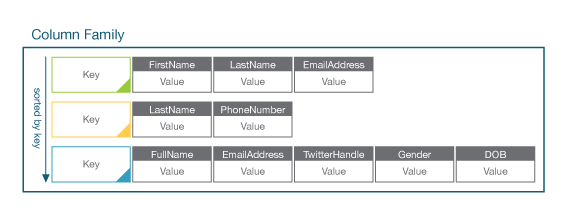
\includegraphics[width=0.8\textwidth]{columns}
		\end{center}
		\caption{Modelagem orientada a colunas}
		\label{fig:mdcolumns}
	\end{figure}


\subsection{Baseados em Grafos}

Nessa categoria os dados são armazenados em nos de um grafo cujas arestas representam o tipo de associação entre esses nós. Esse tipo de banco é especializado em manter dados fortemente ligados. O twitter armazenar as relações entre os seus usuários no seu próprio banco de dados baseados em grafos, o FlockDB, que é otimizado para listas de relações muito grandes, leituras e escritas~\cite{nosqlevaluation}.  Alguns exemplos são: Neo4J, infoGrid e FlockDB~\cite{nosqldatabaseorg}.

\section{MongoDB}


Essa seção foi baseada no site oficial do MongoDB~\cite{sitemongodb} exceto quando explicitamente citado.

MongoDB é um banco de dados NoSQL,  de código aberto,  orientado a documentos, schema-free e escrito em C++.  Os dados são persistidos em coleções de dados que são representados usando o BSON, um formato binário similar ao JSON (Figura \ref{fig:exbson}). O MongoDB tem suporte a todos os tipos de dados  JSON  como string, inteiro, boleano, double, array e objeto. Por usar codificação BSON o MongoDB suporta alguns tipo de dados adicionais como data, binary data, regular expression e code ~\cite{nosqlprofessional}. Na Figura \ref{tab:bytes} podemos ver os tipos suportados pelo BSON.

\begin{table}
	\caption{BSON - Tipos Suportados}
	\begin{center}
	\begin{tabular}{ccc}
		\hline
			\textbf{Tipo} & \textbf{Número} \\
		\hline
			Double & 1 \\
			String & 2 \\
			Object & 3 \\
			Array & 4 \\
			Binary Data & 5 \\
			Object id & 7 \\
			Boolean & 8 \\
			Date & 9 \\
			Null & 10 \\
			Regular Expression & 11 \\
			JavaScript & 13 \\
			Symbol & 14 \\
			JavaScript (with scope) & 15 \\
			32-bit integer & 16 \\
			Timestamp& 17 \\
			64-bit integer & 18 \\
			Min key & 255 \\
			Max key & 127 \\
		\hline
	\end {tabular}
	\end{center}
	%\caption{Fonte: http://docs.mongodb.org}
	\label{tab:bsontypes}
\end{table}

Como não usa o mesmo formato de armazenamento dos SGBDS relacionais, o MongoDB armazena os seus dados em coleções, que são equivalentes às tabelas.  Uma Coleção pode ter um ou mais documentos; são equivalentes as linhas em uma tabela de um banco de dados relacional. Cada documento tem um ou mais campos, o que corresponde a uma coluna.

Diferente do que a maioria das pessoas estão acostumadas, o MongoDB não trabalha com uma estrutura de dados bem definida (schema), ou melhor dizendo, ele usa schemas dinâmicos. Com ele é possível criar coleções sem que a estrutura, campos ou tipos de valores dos documentos estejam definidos. Essa forma flexível de armazenar os dados nos permite trabalhar com estruturas e dados bastante heterogêneos.

	\begin{figure}[!htbp]
		\begin{center}
			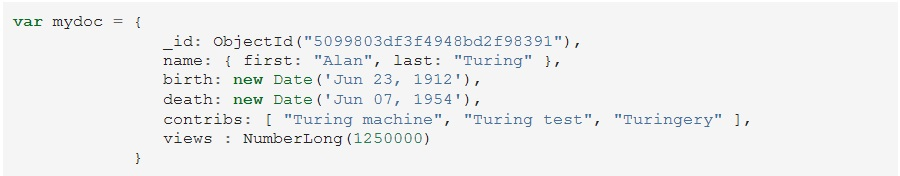
\includegraphics[width=1.2\textwidth]{exbson}
		\end{center}
		\caption{Documento BSON usado no MongoDB}
		%\caption{Fonte: http://docs.mongodb.org}
		\label{fig:exbson}
	\end{figure}

Quanto mais controle, mais custosa é uma operação para o sistema gerenciador de banco de dados.  Os banco de dados NoSQL, como dito anteriormente, foram criados para suprir algumas características que os banco de dados relacionais não atendiam. Uma dessas características é a velocidade com que operações de consulta, escrita, atualização e exclusão são executadas.  Para que a velocidade dessas transações fosse aumentada foi preciso retirar alguns controles, e com isso os banco de dados NoSQL não se comprometem com todas as características ACID.

O MongoDB não provê transações ACID, mas possui alguns recursos transacionais básicos. Operações atômicas são possíveis no escopo de um único documento. Na tabela abaixo temos alguns exemplos de operações em SQL e suas correspondentes no MongoDB.


\section{Cassandra}

Essa seção foi baseada no livro "Cassandra: The Definitive Guide"~\cite{cassandraguide} exceto quando explicitamente citado.

Cassandra é um SGBD NoSQL, de código aberto, do tipo chave-valor e que foi inicialmente desenvolvido pelo Facebook. Com a recente popularização, várias empresas estão achando casos em que o Cassandra pode ser utilizado. Atualmente o Cassandra é usado por por grandes empresas como o Netflix, eBay, Twitter e Cisco~\cite{sitecassandra}. A maior instalação conhecida, com mais de 150 TB e mais de cem máquinas, é a do Facebook.

Cassandra se tornou open-source em julho de 2008 quando o Facebook o mostrou para o mundo e após ser encubado pela apache se tornou bastante popular graças as suas excelentes características técnicas. Ele executa escritas muito rápidas, armazena terabytes de dados e possui uma arquitetura simétrica e descentralizada.

Conforme definido no livro [definitive guide] Apache Cassandra é banco de dados orientado a colunas, open-source, distribuído, de consistência ajustável, descentralizado e elasticamente escalável que é baseado no Amazon Dynamo e no Google Bigtable.

Cassandra representa sua estrutura de dados em tabelas multidimensionais e esparsas (Figura \ref{fig:excassandra}).  No Cassandra podemos ter linhas com uma ou mais colunas, diferentemente de banco de dados relacionais, porem cada linha deve possuir uma chave que a torna acessível. Essa flexibilização do schema nos permite decidir a estrutura de armazenamento da aplicação dinamicamente. Não é preciso saber todas as características e campos do modelo de dados antes do início do projeto.

	\begin{figure}[!htbp]
		\begin{center}
			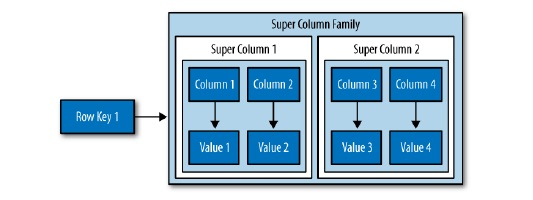
\includegraphics[width=1\textwidth]{excassandra}
		\end{center}
		\caption{Modelo de dados do Cassandra}
		%\caption{Fonte: cassandra guide}
		\label{fig:excassandra}
	\end{figure}

Apesar de ser necessário definir um agrupador chamado keyspace, que contem os aglomerados de colunas, as ‘tabelas’ não precisam de uma definição de quais as colunas vão armazenar. Isso torna o Cassandra schema-free e permite que criemos colunas a qualquer hora. O keyspace é como um namespace lógico que agrupa algumas características e propriedades. 







\section{Testes}

Nessa seção veremos como o teste está diretamente ligado à qualidade de \textit{software}, os principais tipos de testes, conceitos e ferramentas de automação, veremos quais os tipos de testes que serão aplicados ao nosso projeto e a importância da infra-estrutura de testes em um projeto.


\subsection{Definição}

Segundo o dicionário de termos da IEEE, teste é definido da seguinte forma:

\begin{itemize}
	\item Teste: atividades nas quais um sistema ou um componente é executado sob determinadas condições e os resultados são observados ou gravados, e uma avaliação é feita observando determinado comportamento do sistema ou do componente;
\end{itemize}

\subsection{Teste de Software e Qualidade de Software}

O teste de \textit{software} está diretamente ligado com a qualidade do \textit{software} que está sendo desenvolvido. Podemos ver essa ligação já na definição de qualidade de \textit{software}.

\begin{itemize}
	\item Qualidade de \textit{Software}: Conformidade a requisitos funcionais e de desenvolvimento explicitamente declarados, a padrões de desenvolvimento claramente documentados e a características implícitas que são esperadas de todo \textit{software} profissionalmente desenvolvido.
\end {itemize}

Dentro da qualidade de \textit{software} temos a atividade de garantia de qualidade de \textit{software}, e esta compreende uma variedade de tarefas associadas a sete grandes atividades, entre elas a atividade de testes:

\begin{enumerate}
	\item Aplicação de métodos técnicos;
	\item Realização de revisões técnicas formais;
	\item Atividades de testes de \textit{software};
	\item Aplicação de padrões;
	\item Controle de mudanças;
	\item Medição;
	\item Manutenção de registros e reportagem;
\end{enumerate}

Então podemos estar certos de que se queremos um \textit{software} que atenda aos requisitos especificados, funcionais e não funcionais, que possua uma quantidade de erros reduzida e um desempenho que atenda ao usuário, uma tarefa que não pode ser despensada é o teste da aplicação. Como já dito anteriormente, teste de \textit{software} e qualidade de \textit{software} estão intimamente ligados, na tabela ~\ref{tab:testequalidade} podemos ver quais as características de qualidade são verificadas por determinados tipos de testes.

\begin{table}
	\caption{Tipos de teste e sua característica de qualidade correspondente}
	\begin{center}
	\begin{tabular}{ccc}
		\hline
			\textbf{Tipos de Teste} & \textbf{Características de qualidade} \\
		\hline
			Funcionalidade & Funcionalidade \\
			Interfaces & Conectividade \\
			Carga & Continuidade, Performance \\
			Produção & Operabilidade \\
			Recuperação & Recuperação \\
			Regressão id & Todas \\
			Segurança & Segurança \\
		\hline
	\end {tabular}
	\end{center}
	\label{tab:testequalidade}
\end{table}

\subsection{Tipos de Testes}


%Segundo Ian Sommerville, o teste de componentes e o teste de sistema são as duas atividades fundamentais do teste de %software. Enquanto o teste de componentes testa as partes da aplicação, o teste de sistema testa a aplicação como um todo.

O teste de \textit{software} nos permite trabalhar com diversas estratégias e em diferentes níveis da aplicação. Emerson Rios e Trayahú Moreira ~\cite{rios2006teste} dizem que muitas vezes os tipos de \textit{software} se sobrepõem, sendo até mesmo as suas definições abrangentes ou específicas, confome sua execução. Nessa seção listaremos os principais tipos de testes descritos por esses autores.

%\subsubsection{Aplicados a cada estágio de teste}

\begin{description}
\item[Testes Caixa Preta] \hfill \\

Esse tipo de teste tem como objetivo verificar as funcionalidades da aplicação e a aderência aos requisitos, do ponto de vista do usuário, sem se basear no código ou lógica interna da aplicação.

\item[Testes Caixa Branca] \hfill \\

Os testes de caixa branca avaliam o código, a lógica interna do componente, as configurações e outros elementos técnicos.
\end{description}

%\subsubsection{Estágios (ou Níveis) de teste}
\begin{description}
\item[Testes unitários] \hfill \\

Esse é o tipo de teste que analisa o estágio mais baixo da aplicação. São aplicados nos menores componentes de código criados, verificando o atendimento as especificações e funcionalidades. Verificam o funcionamento de um pedaço do sistema, componente ou programa,  isoladamente. Geralmente são realizados pelos próprios desenvolvedores.

\item[Testes de integração] \hfill \\

Esse teste visa testar se as interações estre os componentes da aplicação está resultando em algum tipo de erro. Tem como objetivo assegurar que as interfaces funcionem corretamente e que os dados são processados corretamente.Componentes podem ser pedaços de código, módulos, aplicações distintas, clientes e servidores etc. Esse tipo de teste possui várias estratégias. Podemos testar a integração desde os componentes de mais baixo nível (\textit{Booton-up})  até o sistema como um todo (Teste de sistema). Para o nosso trabalho nos atentaremos ao teste de sistema.

\item[Testes de sistema] \hfill \\

Esse teste é executado sobre o sistema como um todo, ou um subsistema, dentro de um ambiente operacional controlado. Deve ser simulada a operação normal do sistema, sendo testadas todas as suas funções de forma mais próxima possível do que irá ocorrer no ambiente de produção. É nesse estágio que deve-se realizar os testes de carga, performance, usabilidade, compatibilidade, segurança e recuperação.

\item[Testes de aceitação] \hfill \\

São realizados pelos usuários e visam garantir que a solução atenda aos objetivos do negócio e a seus requisitos, verificando as funcionalidades e a usabilidade do \textit{software}.
\end{description}

%\subsubsection{Outros tipos de testes}

\begin{description}

\item[Testes Back-to-back] \hfill \\

É quando o mesmo teste é executado em versões diferentes do \textit{software} e os resultados são comparados.

\item[Testes de Configuração] \hfill \\

É nesse tipo de teste de a execução da aplicação é analisada em diferentes configurações de ambiente.

\item[Testes de Usabilidade] \hfill \\

Mede a facilidade de uso da aplicação pelos usuários. É mais comum em aplicações web.

\item[Testes de Segurança] \hfill \\

Verifica o quão segura é a aplicação a acesso de usuários não autorizados.

\item[Testes de Recuperação] \hfill \\

Mede a qualidade da recuperação do \textit{software} após falhas de \textit{hardware} ou outro problemas inesperados.

\item[Testes de Compatibilidade] \hfill \\

Verifica se um \textit{software} é capaz de ser executado em um ambiente determinado.

\item[Testes de Desempenho] \hfill \\

Verifica a adequação da aplicação aos níveis de desenpenho e tempo de resposta definidos nos requisitos. Também são conhecidos como testes de performance.

\end{description}



\subsection{Testes de Carga e de Performance}

Como o objetivo do trabalho é medir o desempenho da nossa aplicação com o uso de diferentes bancos de dados, restringimos os testes que serão usados no nosso projeto aos testes de carga e performance.

\subsubsection{Testes de carga}

Permite avaliar a aplicação sob uma alta carga de dados, repetidas entradas de dados, consultas complexas ou uma grande quantidade simultânea de usuários. Dessa forma é possível medir o nível de escalabilidade da aplicação. Esse tipo de teste deve ser aplicado durante os testes de sistema e também podem ser chamados de testes de estresse.


\subsubsection{Teste de Performance}

Molyneaux fala que do ponto de vista dos usuários, uma aplicação possui boa performance quando ela o permite realizar determinada tarefa sem demora~\cite{theartoftestperf}. Ela ainda diz que em uma aplicação performática o usuário nunca poderá se deparar com uma tela vazia ao realizar operações. O teste de performance é usado para medir o desempenho, em tempo de execução, e com todos os módulos integrados. Conforme Molyneaux, dividiremos os requisitos de performance em dois: orientados a serviço e orientados a eficiência.

Os indicadores de performance orientados a serviço são a disponibilidade e o tempo de resposta. Eles medem a qualidade do serviço que a aplicação está provendo ao usuário. Já os indicadores orientados a eficiência são a vazão e utilização. Vamos definir esses termos:

\begin{itemize}
\item Disponibilidade: É a característica de estar disponível para o usuário. Em softwares críticos, qualquer período de indisponibilidade pode gerar grandes prejuísos.
\item Tempo de resposta: É o intervalo de tempo entre a requisição e a resposta da aplicação. 
\item Vazão: É a taxa em que os eventos da aplicação ocorrem.
\item Utilização: É a porcentagem da capacidade total de recursos da aplicação que esta sendo usada.
\end{itemize}

Para que o nosso processo de teste de performance seja bem sucedido precisamos seguir algumas etapas.

\begin{enumerate}
\item Escolher uma ferramenta de teste de performance apropriada;
\item Desenvolver um ambiente de teste adequado a realidade dos testes e o mais próximo da realidade;
\item Escolher os objetivos que desejamos alcançar no trabalho;
\item Identificar e criar scripts para as transações críticas para o negócio;
\end{enumerate}


\subsection{Automação de Testes}

Durante muito tempo os testes de \textit{software} foram feitos manualmente. Os proprios programadores eram encarregados de simular as mais diversas situações ~\cite{rios2006teste}. Com o passar do tempo as aplicações se tornaram muito mais complexas e, consequentemente, o processo de teste manual se tornou inviável. Esse cenário foi ideal para que surgissem ferramentas de automação do processo de testes.

	\begin{figure}[!htbp]
		\begin{center}
			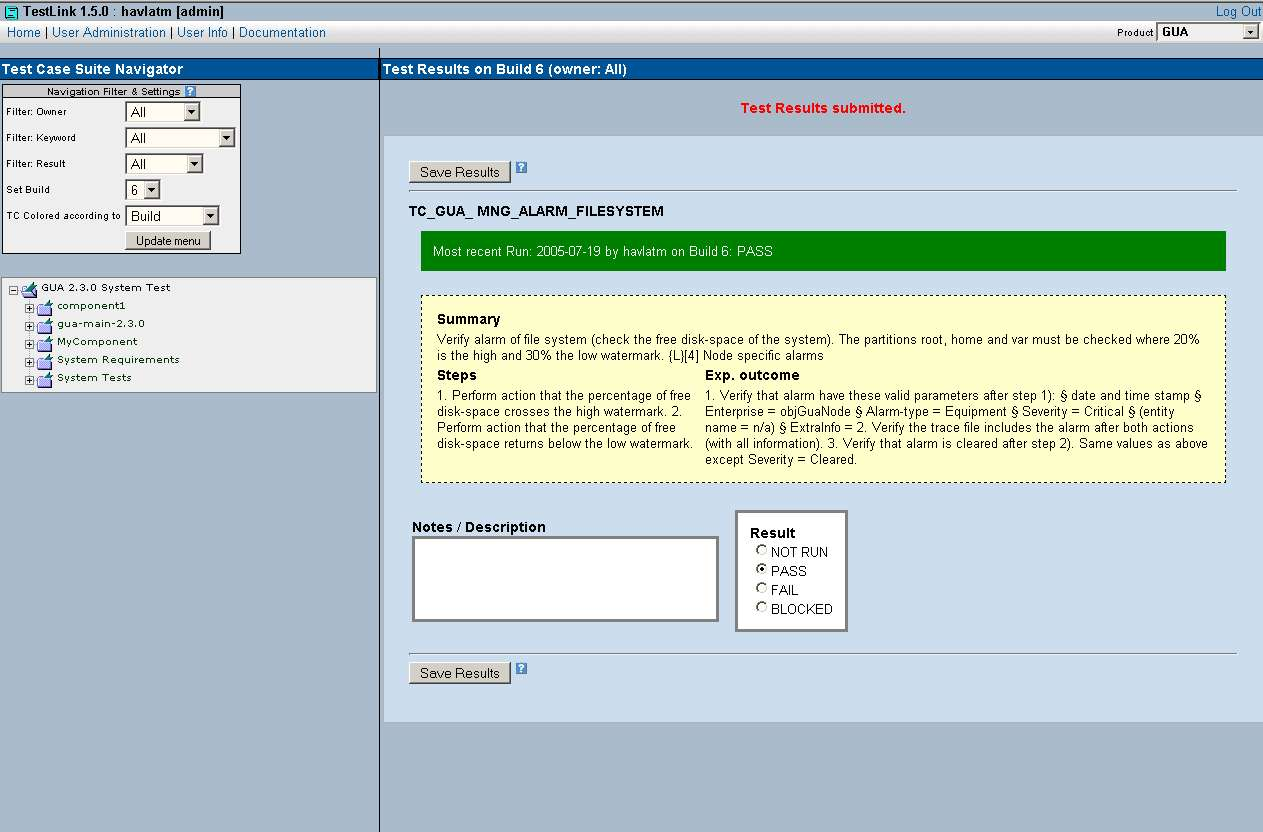
\includegraphics[width=0.8\textwidth]{testlink}
		\end{center}
		\caption{TestLink - acompanhamento/suporte ~\cite{siteTestLink}}
		\label{fig:testlink}
	\end{figure}

As ferramentas de automação de teste visam facilitar o processo de teste e podem auxiliar no desenvolvimento dos testes, execução, manuseio das informações de resultado e a comunicação entre os envolvidos no processo. Utilizando \textit{scripts} essas ferramentas são capazes de simular a utilização da aplicação por um ou vários usuários e, além disso, podem ser simulados vários cenários de uso. As ferramentas de teste podem ser divididas em três grupos: desenvolvimento, execução ~\ref{fig:jmeter} e acompanhamento/suporte ~\ref{fig:testlink}.

	\begin{figure}[!htbp]
		\begin{center}
			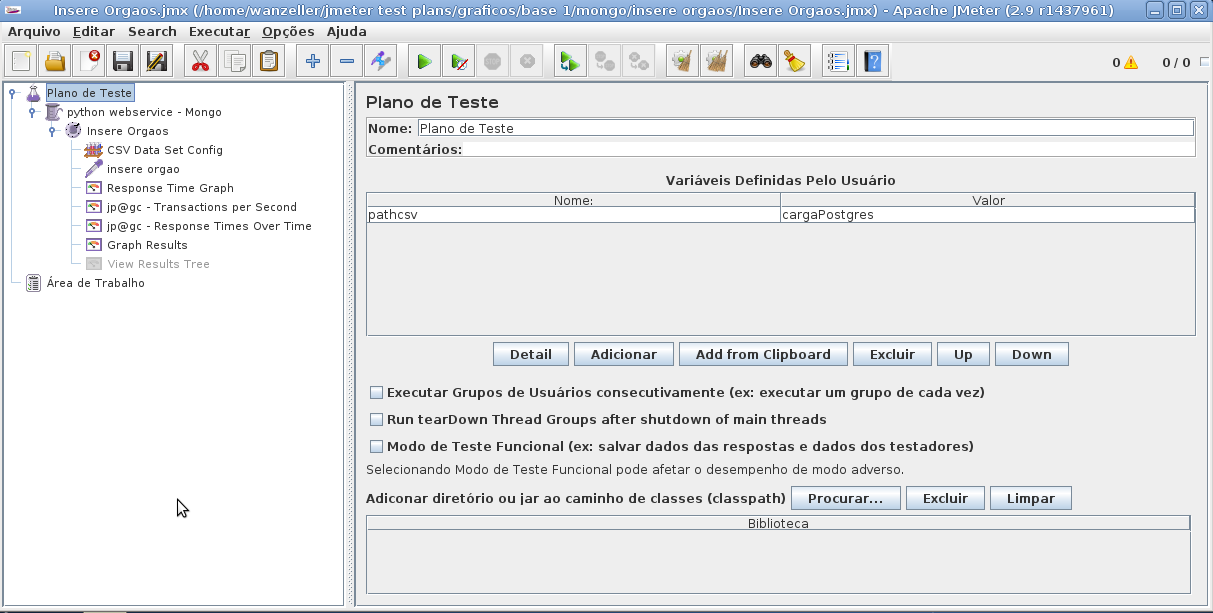
\includegraphics[width=0.8\textwidth]{jmeter}
		\end{center}
		\caption{JMeter - Ferramenta para execução de testes ~\cite{siteJmeter}}
		\label{fig:jmeter}
	\end{figure}


\subsection{JMeter}

O Apache JMeter é uma aplicação \textit{open source}, 100\% desenvolvida em Java e que foi criada para a execução de testes de carca e para medição de performance. Foi originalmente criado para testar aplicações web. O JMeter pode ser usado para testar a performance tanto de recursos estáticos quanto de recursos dinâmicos  (arquivos, servelts, scripts Perl, objetos Java, Bancos de dados e queries, Servidores FTP e etc ). Com ele é possível simular cargas pesadas em um servidor, rede ou objeto para testar o seu comportamento ou para analisar a performance em diferentes tipos de carga ~\cite{siteJmeter}.

O JMeter pode testar diferentes tipos de servidores como:

\begin{itemize}
\item Web - HTTP, HTTPS
\item SOAP
\item Database via JDBC
\item LDAP
\item JMS
\item Mail - SMTP, POP3 e IMAP
\item Comandos nativos ou scripts shell
\end{itemize}

Para realizarmos testes no JMeter precisamos criar um plano de teste. O plano de teste descreve uma série de passos que o JMeter terá de executar. O plano de teste pode conter os seguintes elementos: Grupo de Thread, controladores lógicos, testadores, ouvintes, \textit{timers}, \textit{assertions} e elementos de configuração. A seguir vamos ver os elementos que serão usados nos planos de teste desse trabalho.

Quando iniciamos o nosso plano de teste, o primeiro item que devemos procurar é o testador. Os testadores basicamente enviam requisições aos servidores e aguardam retorno. Cada testador possui diversas configurações que podem ser customizadas.

\begin{description}
\item[ Testador de Requisição SOAP/XML - RPC] \hfill \\

O testador SOAP (figura \ref{fig:testador_insere_orgao}) é usado para mandar requisições SOAP para um Web service.  Ele cria uma requsição HTTP POST com os dados especificados e executa o POST.  As principais configurações são:


\begin{itemize}
\item \textbf{URL}:  Endereço do WSDL do Web service.
\item \textbf{Ação SOAP}: Endereço da requisição SOAP que o testador utilizará.
\item \textbf{Dados SOAP/XML-RPC}: Requisição que será enviada para o Web service. Deve estar em formato XML.
\end{itemize}

	\begin{figure}[!htbp]
		\begin{center}
			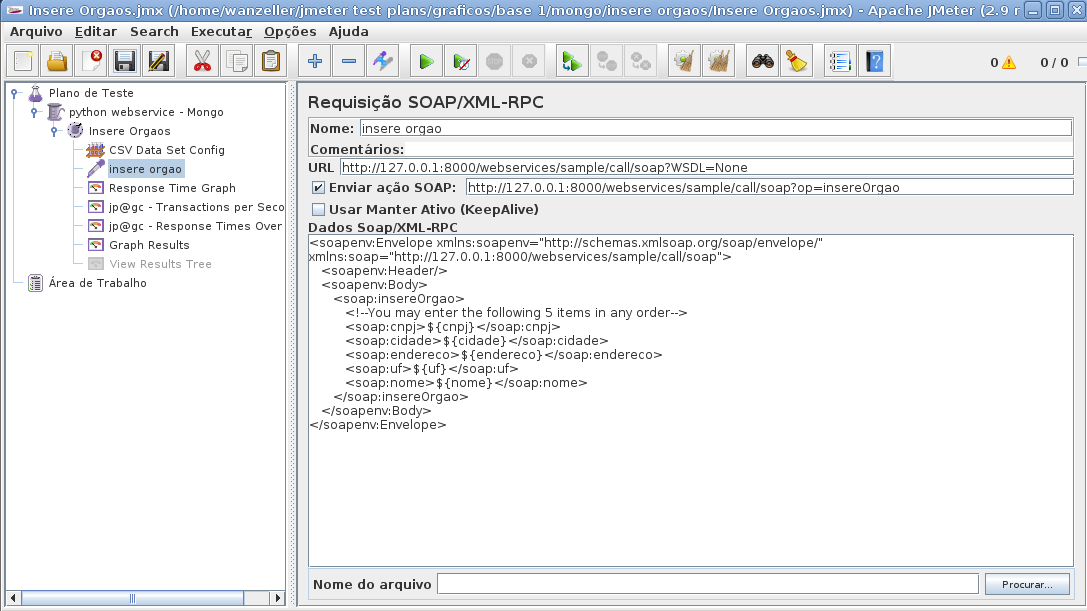
\includegraphics[width=1\textwidth]{testador_insere_orgao}
		\end{center}
		\caption{Testador de Requisição SOAP/XML - RPC}
		\label{fig:testador_insere_orgao}
	\end{figure}
	
\end{description}

Os ouvintes nos permite ter acesso às informações geradas pelo JMeter durante os testes. Temos ouvintes que geram gráficos, gravam informações em arquivos, listam o retorno das requisições e outros vários. A seguir veremos o gráfico de resultados e o gráfico de tempo de resposta.

\begin{description}
\item[Gráfico de Resultados] \hfill \\

O gráfico de resultados gera um gráfico com os tempos de todas as requisições. Na legenda do gráfico temos o tempo da requisição atual (preto), a média atual de todas as requisições (azul), a derivação atual (vermelho), e a vazão atual (verde), todas em milisecundos. A vazão representa o número de transações por minuto (os atrazos causados pelo processamento interno do JMeter não são considerados).

\item[Gráfico de Tempo de Resposta] \hfill \\

O gráfico de tempo de resposta plota uma linha no gráfico que descreve a evolução do tempo de resposta de cada requisição durante o teste.
\end{description}

Os elementos de configuração podem ser utilizadoos para configurar padrões e variáveis que serão utilizadas pelos testadores.

\begin{description}
\item[Elemento para Configuração de Dados CSV] \hfill \\

Esse elemento de configuração é usado para ler linhas de um arquivo e armazená-las em variáveis.Podemos ver um exemplo na figura \ref{fig:configuracao_csv}. Para realizar os testes de inserção de dados no banco esse elemento será de grande importância.

	\begin{figure}[!htbp]
		\begin{center}
			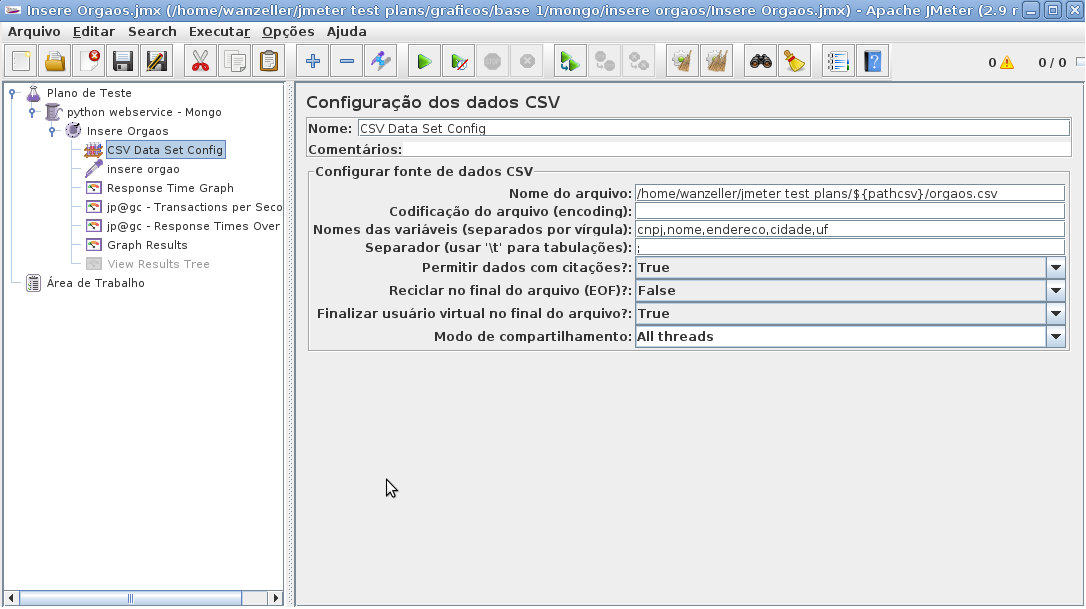
\includegraphics[width=1\textwidth]{configuracao_csv}
		\end{center}
		\caption{Elemento de Configuração de Dados CSV}
		\label{fig:configuracao_csv}
	\end{figure}
	
\end{description}















\section{Web-Service}


Nessa seção daremos uma visão de o que é \textit{web service}, e mostraremos um pouco sobre os seus principais componentes. Essa seção foi baseado no w3c schools ~\cite{w3cs} exeto quando citado explicitamente.

\subsection{O que é web-service?}

\textit{Web service} são componentes que podem ser acessados via protocolo http. Atualmente é muito usado na comunicação entre aplicações diferentes. O acesso a um \textit{web service} é via http, mas internamente existe dados formatados em xml que estão empacotados no protocolo SOAP (Simple Object Access Protocol).

Hoje várias aplicações podem acessar a web usando os \textit{browsers} e nem sempre essas aplicações conversam entre si. Para que a comunicação entre essas diversas aplicações se tornasse possível, independente da plataforma em que estivessem desenvolvidas, foi criado o conceito de \textit{web service}. Usando \textit{web services}, as aplicações podem publicar suas funções para toda a web. Usando o XML para codificar e SOAP para transportar os dados, os \textit{web services} elevaram as aplicações web para outro nível.

\subsection{Componentes de um Web-Service}

Um \textit{web service} é formado por três elementos: SOAP, WSDL e UDDI.

\subsubsection{SOAP}


O SOAP (Simple Object Access Protoco) é um protocolo leve para troca de informações que foi criado pela Microsoft, Ariba e IBM para padronizar a transferência de dados em diversas aplicações, por isso, se dá em XML. Parte da sua especificação é composta por um conjunto de regras de como utilizar o XML para representar os dados. Outra parte define o formato de mensagens, convenções para representar as chamadas de procedimento remoto (RPCs) utilizando o SOAP, e associações ao protocolo HTTP. 

SOAP é:

\begin{itemize}
	\item Um protocolo de comunição;
	\item É usado para a comunicação entre aplicações;
	\item É um padrão para envio de mensagens;
	\item Sua comunicação se dá na internet;
	\item É independente de plataforma;
	\item É independente de linguagem de programação;
	\item É baseado em XML;
	\item Permite passar por \textit{firewalls};
	\item É uma recomendação do W3C;
\end{itemize}

Atualmente as aplicações se comunicam via RPC (Remote Procedure Calls), mas o HTTP não foi desenhado para isso. RPC possui problemas de compatibilidade e segurança; \textit{firewalls} e servidores de \textit{proxy} normalmente bloqueiam mensagens desse tipo. Para resolver esses problemas foi criado o protocolo SOAP.

Uma mensagem SOAP (Exemplo \ref{listing:msgsoap}) é basicamente um documento XML que contem os seguintes elementos:

\begin{itemize}
	\item Um elemento 'Envelope' que identifica o documento XML como uma mensagem SOAP;
	\item Um elemento 'header' que contem informações de cabeçalho;
	\item Um elemento 'body' que contem informações de chamadas e retornos;
	\item Um elemento 'Fault' que contem informações sobre erros e status;
\end{itemize}


\definecolor{gray}{rgb}{0.4,0.4,0.4}
\definecolor{darkblue}{rgb}{0.0,0.0,0.6}
\definecolor{cyan}{rgb}{0.0,0.6,0.6}

\lstset{
  basicstyle=\ttfamily,
  columns=fullflexible,
  showstringspaces=false,
  commentstyle=\color{gray}\upshape
}

\lstdefinelanguage{XML}
{
  morestring=[b]",
  morestring=[s]{>}{<},
  morecomment=[s]{<?}{?>},
  stringstyle=\color{black},
  identifierstyle=\color{darkblue},
  keywordstyle=\color{cyan},
  morekeywords={xmlns,version,type}% list your attributes here
}


\lstset{language=XML}
\begin{lstlisting}[caption={Estrutura de uma mensagem SOAP},frame=trBL,breaklines=true,label=listing:msgsoap]
<?xml version="1.0"?>

<soap:Envelope
xmlns:soap="http://www.w3.org/2001/12/soap-envelope"
soap:encodingStyle="http://www.w3.org/2001/12/soap-encoding">

<soap:Header>
...
</soap:Header>

<soap:Body>
...  
	<soap:Fault>
	  ...  
	</soap:Fault>
</soap:Body>

</soap:Envelope>
\end{lstlisting}

\subsection{WSDL}

WSDL é uma linguagem baseada em XML para localizar e descrever \textit{web services}.

O WSDL (\textit{Web Services Description Language}) é uma linguagem baseada em XML, com a finalidade de documentar as mensagens que o Web service aceita e gera (Exemplo \ref{listing:wsdl}). É uma espécie de contrato. Esse mecanismo padrão facilita a interpretação dos 'contratos' pelos desenvolvedores e ferramentas de desenvolvimento. 

WSDL é:

\begin {itemize}
	\item A linguagem padrão para descrever \textit{web services};
	\item É baseado em XML;
	\item É usado para localizar \textit{web services};
	\item É um padrão W3C.
\end {itemize}

Um WSDL descreve um \textit{web service} usando pricipalmente os seguintes elementos:

\begin{table}[h]
	\caption{Elementos de um documento WSDL}
	\begin{center}
	\begin{tabular}{ccc}
		\hline
			\textbf{Elemento} & \textbf{Descrição} \\
		\hline
			<types> & Um container para a definição dos tipos de dados usados pelo \textit{web service}\\
			<message> & Definição dos dados que serão usados na comunicação \\
			<portType> & Um conjunto de operações suportadas por um ou mais \textit{endpoints} \\
			<binding> & Um protocolo e especificação de dados para um \textit{port type} específico\\
		\hline
	\end {tabular}
	\end{center}
	%\{Fonte: http://www.w3schools.com/}
	\label{tab:elementosWsdl}
\end{table}

Abaixo temos uma fração simplificada de um documento WSDL:

\lstset{language=XML}
\begin{lstlisting}[caption={WSDL},frame=trBL,breaklines=true,label=listing:wsdl]
<message name="getTermRequest">
  <part name="term" type="xs:string"/>
</message>

<message name="getTermResponse">
  <part name="value" type="xs:string"/>
</message>

<portType name="glossaryTerms">
  <operation name="getTerm">
    <input message="getTermRequest"/>
    <output message="getTermResponse"/>
  </operation>
</portType> 
\end{lstlisting}

\subsection{UDDI}

UDDI é um serviço de diretório que permite às empresas descobrir, registrar e procurar \textit{web services}. É baseado em padrões do W3C (\textit{World Wide Web Consortium}) e IETF (\textit{Internet Task Force}) como XML, HTTP e DNS.

Os benefícios de se usar UDDI são muitos. Antes do UDDI não havia padrão para as empresas divulgarem seus produtos e serviços para os seus consumidores e parceiros. Com o UDDI, por exemplo, se for definido um padrão para serviços de empresas aéreas, quando as empresas publicarem os seus serviços em um diretório UDDI as agências de viagem poderão procurar por esses serviços e iniciar imediatamente a comunicação.















   